\documentclass{article}
\usepackage{tikz, comment}
\usepackage{pifont}
\usepackage{fontspec}
\usetikzlibrary{arrows, decorations.markings, decorations.pathreplacing}
\begin{comment}
:Title: Not defined yet
:Tags: foci of an ellipse;ellipse;perimeter;focal radius ;focus of a parabola
:Prob: 0.5282;0.5142;0.4273;0.422;0.4086
:Author: Prof.Hu Ji-shan, HKUST
:Slug: No name yet

Description Here.........
\end{comment}
\begin{document}\centering

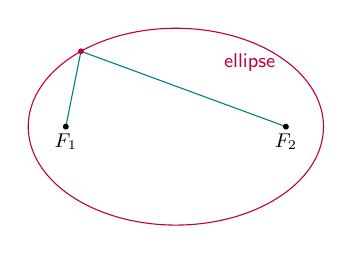
\begin{tikzpicture}[>=latex,xscale=.5*1.25, yscale=.5*1.25][font=\sf\small]

\draw[purple, samples=100, smooth, domain=0:2*pi, variable=\t]
plot ({3*cos(\t r)}, {2*sin(\t r)}) ;

\node[purple, scale=0.8] at (1.5, 1.3) {$\hbox{ellipse}$};

\draw[teal] ({-sqrt(5)}, 0) -- ({3*cos(130)}, {2*sin(130)}) -- ({ sqrt(5)}, 0);

\draw[fill, xscale=1/1.25, yscale=1/1.25] ({-sqrt(5)*1.25}, 0) circle(0.06) node[below, scale=0.8]{$F_1$};
\draw[fill, xscale=1/1.25, yscale=1/1.25] ({ sqrt(5)*1.25}, 0) circle(0.06) node[below, scale=0.8]{$F_2$};
\draw[purple, fill, xscale=1/1.25, yscale=1/1.25] ({3*cos(130)*1.25}, {2*sin(130)*1.25}) circle(0.06);

\end{tikzpicture}
\end{document}